% Tento soubor nahraďte vlastním souborem s obsahem práce.
%=========================================================================
% Autoři: Michal Bidlo, Bohuslav Křena, Jaroslav Dytrych, Petr Veigend a Adam Herout 2019

% Pro kompilaci po částech (viz projekt.tex), nutno odkomentovat a upravit
%\documentclass[../projekt.tex]{subfiles}
%\begin{document}

\chapter{Úvod}

Se stále rostoucí závislostí dnešní společnosti na internetu a počítačích se z těchto technologií stala neodmyslitelná součást našich životů. 
Ovšem stále častěji jsou tyto technologie zneužívány útočníky, kteří přicházejí stále s novými metodami, jak napadnou počítače uživatelů a narušit tak jejich soukromý a nebo odcizit citlivé informace.
Proto je nutné, aby prostředky pro boj s těmito útoky byly neustále modernizovány a byly co nejúčinější.

Proto programy pro detekci škodlivého softwaru (z anglického malicious software, dále pak už jen zkráceně malware) založené na strojovém učení, které jsou v současné době využívány, vyžadují vhodnou datovou sadu na které se bude model učit a ověřovat svoji validitu.
Cílem této práce tedy je vytvoření vhodného nástroje na tvorbu datových sad, které jsou nezbytné pro tyto metody. %detekce založené na strojovém učení.
A dále je pak porovnání těchto metod a jejich úspěšnosti při detekci škodlivého softwaru.

Hlavním důvodem, proč se zabývat rozpoznáváním jednotlivých druhů malwaru a jejich klasifikací, je jeho nezbytnost a důležitost.
Jelikož je velice nereálné, že by v následujícíh letech vymizela potřeba se před těmito útoky branít. Ba naopak lze předpokládat, že 
bude příbývat stále více nových druhů škodlivého softwaru, a proto je nutné na tyto změny rychle a efektivně reagovat, aby byla zajištěna
bezpečnost uživatelů internetových sítí.

Tato bakalářská práce se skláda ze 4 kapitol. Toho úvodu, který slouží jako nahlédnutí do problematiky, následují dvě samostatné kapitoly a závěru. V kapitola \ref{2.chap} se nejprve seznámíte s dělení škodlivého softwaru do rodin. Následně
je představeno několik současných řešení detekce škodlivého softwaru, které jsou založeny na strojovém učení a jejich údajná přesnost.
V kapitole s číslem \ref{3.chap} je pak přiblížen způsob jakým byly vytvořeny vhodné datové sady a popis vytvořeného nástroje sloužícího k tomuto účelu. V závěru jsou pak zhodnoceny dosavadní výsledky a postup další práce.

\chapter{Malware} \label{2.chap}
%Prejmenovat tuto kapitolu
Cca 8 stranky co to vůbec malware je a jak se deli a jaké způsoby na detekci se v současné době používají.
Příklady rodin a nějaké statistiky.


\chapter{Automatická tvorba datasetů} \label{3.chap}
Proč jsou datasety důležité, popsat můj nástroj na tvorbu datasetů. Co je jeho výstupem a jak funguje.

Podstatnou a velice důležitou částí této práce je výběr a tvorba vhodných datových sad (z anglického \textit{datasets}), jelikož s daty souvisí důveryhodnost dosažených výsledků.


Obrázek jednoduché pipeline.

\begin{figure}[h]
	\centering
        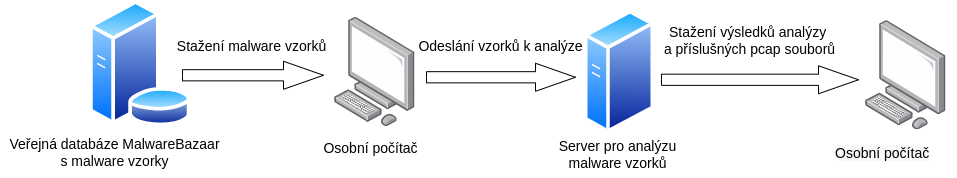
\includegraphics[width=0.8\textwidth]{obrazky/pipeline.png}
	\caption{Proces tvorby datasetů}
    \label{pipeline}
\end{figure}

Cca 5 stranek
    
\chapter{Závěr}
Max 1 stranka \cite{Pysny}

TODO



%===============================================================================

% Pro kompilaci po částech (viz projekt.tex) nutno odkomentovat
%\end{document}
